
\section{\trTensor{}与\trCotensor}\label{sec:tensors-and-cotensors}

一个 $\mathcal{V}$-范畴 $\mathcal{C}$ 容有\emph{张量}（tensors），恰当时对一切
$c\in\mathcal{C}$，协变可表示函子
$\mathcal{C}(c,-)\colon\mathcal{C}\to\mathcal{V}$ 容有一个左 $\mathcal{V}$-伴随
$-\otimes c\colon\mathcal{V}\to\mathcal{C}$。对偶地，一个 $\mathcal{V}$-范畴
$\mathcal{C}$ 容有\emph{余张量}（cotensors），恰当时反变可表示函子
$\mathcal{C}(-,c)\colon\mathcal{C}^{\mathrm{op}}\to\mathcal{V}$ 容有一个与之
互为右 $\mathcal{V}$-伴随
$c^{-}\colon\mathcal{V}^{\mathrm{op}}\to\mathcal{C}$。本节的目标是把这两种构造
形式化地引入。我们将会发现，当把诸富集范畴的诸底范畴之间的诸\trFunctor{}加以
富集时，张量或余张量的存在是有用的。

\begin{definition}\label{def:cotensored}
一个 $\mathcal{V}$-范畴 $\mathcal{C}$ 是\textbf{余张量化的}（cotensored），若
对一切 $v\in\mathcal{V}$ 与 $c\in\mathcal{C}$，$\mathcal{V}$-函子
$\mathcal{C}(-,c)^{v}\colon\mathcal{C}^{\mathrm{op}}\to\mathcal{V}$ 被一个对象
$c^{v}\in\mathcal{C}$ 所表示，意即存在一个\trIsomorphism
\[ \mathcal{C}(x,c^{v})\cong\mathcal{C}(x,c)^{v} \]
居于 $\mathcal{V}$ 之中并且在 $x$ 上是 $\mathcal{V}$-自然的。由\cref{prop:unique-extension-vfunctor}，
余张量积定义一个唯一的 $\mathcal{V}$-函子
\[ \mathcal{C}\times\mathcal{V}^{\mathrm{op}}
   \xrightarrow{\ (-)^{-}\ }\mathcal{C} \]
使得定义性\trIsomorphism{}在所有三个变量上都是 $\mathcal{V}$-自然的。
\end{definition}

\begin{definition}\label{def:tensored}
对偶地，一个 $\mathcal{V}$-范畴 $\mathcal{C}$ 是\textbf{张量化的}
（tensored），若对一切 $v\in\mathcal{V}$ 与 $c\in\mathcal{C}$，$\mathcal{V}$-函子
$\mathcal{C}(c,-)^{v}\colon\mathcal{C}\to\mathcal{V}$ 被一个对象
$v\otimes c\in\mathcal{C}$ 所表示，意即存在一个\trIsomorphism
\[ \mathcal{C}(v\otimes c,x)\cong\mathcal{C}(c,x)^{v} \]
居于 $\mathcal{V}$ 之中并且在 $x$ 上是 $\mathcal{V}$-自然的。由\cref{prop:unique-extension-vfunctor}，
\trTensorProduct{}定义一个唯一的 $\mathcal{V}$-函子
\[ \mathcal{V}\times\mathcal{C}\xrightarrow{\ -\otimes-\ }\mathcal{C} \]
使得定义性\trIsomorphism{}在所有三个变量上都是 $\mathcal{V}$-自然的。
\end{definition}

直接从这些定义可得：

\begin{lemma}\label{lem:tensored-cotensored-two-variable-adjunction}
一个 $\mathcal{V}$-范畴 $\mathcal{C}$ 是张量化且余张量化的，当且仅当
$\mathcal{V}$-函子
$\mathcal{C}(-,-)\colon\mathcal{C}^{\mathrm{op}}\times\allowbreak\mathcal{C}\to\allowbreak\mathcal{V}$
参与一个双变量 $\mathcal{V}$-伴随
\[
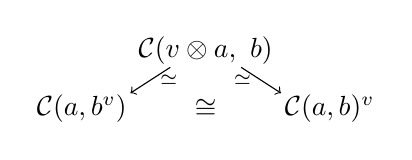
\begin{tikzpicture}[x=1.6em,y=1.5em]
  \node (t)  at (2.8,1.4) {$\mathcal{C}(v\otimes a,\ b)$};
  \node (bl) at (0,0)   {$\mathcal{C}(a,b^{v})$};
  \node (br) at (5.6,0) {$\mathcal{C}(a,b)^{v}$};
  \draw[->] (2.0,1.0) -- node[right]{$\scriptstyle\simeq$} (1.1,0.38);
  \draw[->] (3.6,1.0) -- node[left]{$\scriptstyle\simeq$} (4.5,0.38);
  \node at (2.8,0) {$\cong$};
\end{tikzpicture}
\]
一如这个由 $\mathcal{V}$-自然\trIsomorphism{}组成的交换三角形所表达。%
\footnote{原书此处三角形顶点印作「$\mathcal{C}(v\times a,\ b)$」；按
$v\in\mathcal{V}$、$a\in\mathcal{C}$，笛卡尔积不合型，依定义 A.4.2 之张量
同构 $\mathcal{C}(v\otimes c,x)\cong\mathcal{C}(c,x)^{v}$，疑为张量
$v\otimes a$ 之误，此处径改。——译者注}
\end{lemma}

定义性自然\trIsomorphism{}的 $\mathcal{V}$-自然性有如下推论：

\begin{lemma}\label{lem:tensor-cotensor-unit-associativity}
在任何富集于 $\mathcal{V}$ 之上且余张量化的\trCategory{} $\mathcal{C}$ 中，
存在 $\mathcal{V}$-自然\trIsomorphism
\[ c^{1}\cong c
   \qquad\text{以及}\qquad
   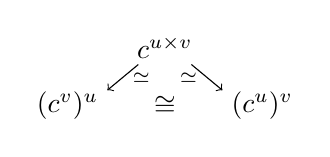
\begin{tikzpicture}[x=1.6em,y=1.5em]
     \node (t)  at (2.2,1.4) {$c^{u\times v}$};
     \node (bl) at (0,0)   {$(c^{v})^{u}$};
     \node (br) at (4.4,0) {$(c^{u})^{v}$};
     \draw[->] (1.6,1.0) -- node[right]{$\scriptstyle\simeq$} (0.9,0.38);
     \draw[->] (2.8,1.0) -- node[left]{$\scriptstyle\simeq$} (3.5,0.38);
     \node at (2.2,0) {$\cong$};
   \end{tikzpicture} \]
对 $u,v\in\mathcal{V}$ 与 $c\in\mathcal{C}$。对偶地，若 $\mathcal{C}$ 富集于
$\mathcal{V}$ 之上且是张量化的，则存在 $\mathcal{V}$-自然\trIsomorphism
\[ 1\otimes c\cong c
   \qquad\text{以及}\qquad
   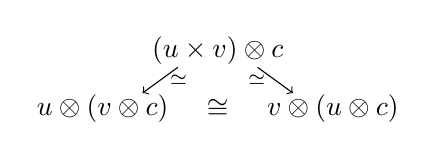
\begin{tikzpicture}[x=1.6em,y=1.5em]
     \node (t)  at (2.6,1.4) {$(u\times v)\otimes c$};
     \node (bl) at (0,0)   {$u\otimes(v\otimes c)$};
     \node (br) at (5.2,0) {$v\otimes(u\otimes c)$};
     \draw[->] (1.7,1.0) -- node[right]{$\scriptstyle\simeq$} (0.9,0.38);
     \draw[->] (3.5,1.0) -- node[left]{$\scriptstyle\simeq$} (4.3,0.38);
     \node at (2.6,0) {$\cong$};
   \end{tikzpicture} \]
对 $u,v\in\mathcal{V}$ 与 $c\in\mathcal{C}$。
\end{lemma}

在这些 $\mathcal{V}$-自然\trIsomorphism{}之间存在种种相干关系，它们源自%
\trCartesianClosed{}\trCategory{} $\mathcal{V}$ 的诸相干关系。

\begin{proof}
由\cref{lem:isomorphism-characterizations}，为定义所显示的那些\trIsomorphism，只需证明这些对象表示同一个
$\mathcal{V}$-函子 $\mathcal{C}^{\mathrm{op}}\to\mathcal{V}$。由余张量的定义性%
\trUniversalProperty，对任何 $x\in\mathcal{C}$，存在 $\mathcal{V}$-自然%
\trIsomorphism
\[ \mathcal{C}(x,c^{1})\cong\mathcal{C}(x,c)^{1}\cong\mathcal{C}(x,c), \]
最后一个\trIsomorphism{}由注 A.1.9（\cref{rem:exponent-one-identity}）给出。
由于这些\trIsomorphism{}在 $c$ 上与在 $x$ 上一样是 $\mathcal{V}$-自然的，
\trIsomorphism{} $c^{1}\cong c$ 也是 $\mathcal{V}$-自然的。

类似地，在下方三角形的三个顶点处各存在 $\mathcal{V}$-自然\trIsomorphism
\begin{center}
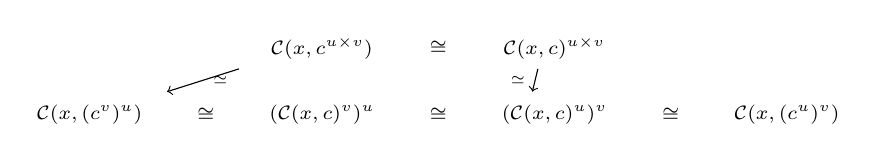
\begin{tikzpicture}[x=1.0em,y=1.5em,every node/.style={font=\scriptsize}]
  \node (T1) at (8.4,1.6) {$\mathcal{C}(x,c^{u\times v})$};
  \node at (12.6,1.6) {$\cong$};
  \node (T2) at (16.8,1.6) {$\mathcal{C}(x,c)^{u\times v}$};
  \node (B1) at (0,0) {$\mathcal{C}(x,(c^{v})^{u})$};
  \node at (4.2,0) {$\cong$};
  \node (B2) at (8.4,0) {$(\mathcal{C}(x,c)^{v})^{u}$};
  \node at (12.6,0) {$\cong$};
  \node (B3) at (16.8,0) {$(\mathcal{C}(x,c)^{u})^{v}$};
  \node at (21.0,0) {$\cong$};
  \node (B4) at (25.2,0) {$\mathcal{C}(x,(c^{u})^{v})$};
  \draw[->] (5.4,1.1) -- node[right]{$\scriptstyle\simeq$} (2.8,0.55);
  \draw[->] (16.2,1.1) -- node[left]{$\scriptstyle\simeq$} (16.0,0.55);
\end{tikzpicture}
\end{center}
其中起连接作用的诸 $\mathcal{V}$-自然\trIsomorphism{}由引理 A.1.7
（\cref{lem:isos-lift-to-V}）给出。再者，这些\trIsomorphism{}在 $u$、$v$ 与
$c$ 上的 $\mathcal{V}$-自然性给出了所述陈述的 $\mathcal{V}$-自然性。
\end{proof}

推广\cref{lem:cartesian-closed-v-category}：

\begin{lemma}\label{lem:cartesian-closed-self-tensored}
一个\trCartesianClosed{}\trCategory{} $(\mathcal{V},\times,1)$ 富集、张量化且
余张量化于其自身之上，其中张量由笛卡尔积定义，而余张量则由%
\trInternalHom\footnote{这为\trInternalHom{}与余张量二者对指数记号的滥用提供了
开脱。}定义：
\[ v\otimes w\coloneqq v\times w
   \qquad\text{以及}\qquad
   w^{v}\coloneqq w^{v}. \]
\end{lemma}

\begin{proof}
引理 A.1.7（\cref{lem:isos-lift-to-V}）在 $\mathcal{V}$ 中确立了所需的那些%
\trIsomorphism
\eqref{eq:associativity-triangle-isos}。其 $\mathcal{V}$-自然性的证明留给
读者，或见 \cite[\S\,1.8]{bib68}。
\end{proof}

现在考虑一个 $\mathcal{V}$-函子 $F\colon\mathcal{C}\to\mathcal{D}$。若
$\mathcal{C}$ 与 $\mathcal{D}$ 都张量化于 $\mathcal{V}$ 之上，则复合映射
\[ v\xrightarrow{\ \eta_{v}\ }\mathcal{C}(c,v\otimes c)
   \xrightarrow{\ F_{c,v\otimes c}\ }\mathcal{D}(Fc,F(v\otimes c)) \]
经转置而定义一个\trCanonical{} $\mathcal{V}$-\trNaturalTransformation{}
$\tau_{v,c}\colon v\otimes Fc\to F(v\otimes c)$。若此映射是 $\mathcal{D}$ 中的
一个\trIsomorphism，则称 $\mathcal{V}$-函子 $F$ \textbf{保持张量}（preserves
tensors）。

张量与余张量的存在提供了一种便利的机制，用以检验一个先验非富集的%
\trAdjunction{}可否被富集成一个 $\mathcal{V}$-伴随。

\begin{proposition}\label{prop:enriched-adjoint-preserves-tensors}
设 $\mathcal{A}$ 与 $\mathcal{B}$ 是 $\mathcal{V}$-范畴。
\begin{enumerate}[label=(\roman*)]
\item 若 $\mathcal{A}$ 与 $\mathcal{B}$ 张量化于 $\mathcal{V}$ 之上，则一个
  $\mathcal{V}$-函子 $F\colon\mathcal{B}\to\mathcal{A}$ 是一个左
  $\mathcal{V}$-伴随，当且仅当 $F$ 容有一个非富集右伴随并且保持张量。
\item 若 $\mathcal{A}$ 与 $\mathcal{B}$ 余张量化于 $\mathcal{V}$ 之上，则一个
  $\mathcal{V}$-函子 $U\colon\mathcal{A}\to\mathcal{B}$ 是一个右
  $\mathcal{V}$-伴随，当且仅当 $U$ 容有一个非富集左伴随并且保持余张量。
\end{enumerate}
\end{proposition}

\begin{proof}
我们对这对对偶陈述中的第一条证明诸条件的充分性，而把它们的必要性留给%
\cref{ex:enriched-left-adjoints-preserve-tensors}。设 $F$ 容有一个带%
\trCounit{} $\varepsilon$ 的非富集右伴随 $U$。由\cref{exa:post-composition-vnatural-transformation}与\cref{ex:functor-arrow-vnatural}，
$\mathcal{V}$ 中 hom-对象的如下复合映射
\begin{rveq}\label{eq:adjunction-composite}
\mathcal{B}(b,Ua)\xrightarrow{\ F_{b,Ua}\ }\mathcal{A}(Fb,FUa)
   \xrightarrow{\ \varepsilon_{a\circ-}\ }\mathcal{A}(Fb,a)
\end{rveq}
——它提升该非富集\trAdjunction{}的 hom-集双射——在 $b$ 上是 $\mathcal{V}$-自然的。
我们的任务是证明 \eqref{eq:adjunction-composite} 是 $\mathcal{V}$ 中的一个%
\trIsomorphism。此后由\cref{prop:unique-extension-vfunctor}，存在唯一的方式把右伴随 $U$ 富集起来，使得
这个映射在 $a$ 上与在 $b$ 上一样是 $\mathcal{V}$-自然的。

在施加非富集可表示函子
$\mathcal{V}(v,-)\colon\mathcal{V}\to\mathcal{S}et$ 之后，我们声称：此映射可
嵌入如下交换图表之中
\begin{center}
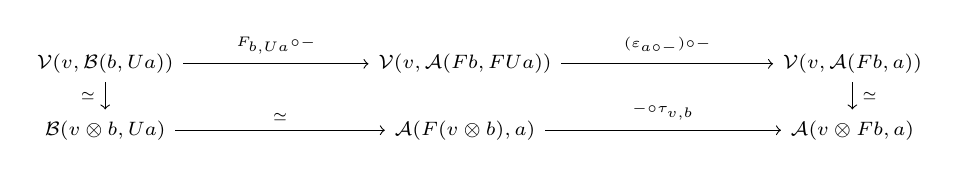
\begin{tikzpicture}[x=1.0em,y=1.5em,every node/.style={font=\scriptsize}]
  \node (TL) at (0,1.6) {$\mathcal{V}(v,\mathcal{B}(b,Ua))$};
  \node (TM) at (13.0,1.6) {$\mathcal{V}(v,\mathcal{A}(Fb,FUa))$};
  \node (TR) at (27.0,1.6) {$\mathcal{V}(v,\mathcal{A}(Fb,a))$};
  \node (BL) at (0,0) {$\mathcal{B}(v\otimes b,Ua)$};
  \node (BM) at (13.0,0) {$\mathcal{A}(F(v\otimes b),a)$};
  \node (BR) at (27.0,0) {$\mathcal{A}(v\otimes Fb,a)$};
  \draw[->] (TL) -- node[above]{$\scriptstyle F_{b,Ua}\circ-$} (TM);
  \draw[->] (TM) -- node[above]{$\scriptstyle(\varepsilon_{a\circ-})\circ-$} (TR);
  \draw[->] (0,1.15) -- node[left]{$\scriptstyle\simeq$} (0,0.5);
  \draw[->] (27.0,1.15) -- node[right]{$\scriptstyle\simeq$} (27.0,0.5);
  \draw[->] (BL) -- node[above]{$\scriptstyle\simeq$} (BM);
  \draw[->] (BM) -- node[above]{$\scriptstyle-\circ\tau_{v,b}$} (BR);
\end{tikzpicture}
\end{center}
其中那三个\trIsomorphism{}由跨越非富集\trAdjunction{}作转置而定义。由于这是
一个由集合之间的函数构成的图表，为验证其交换性，只需考虑一个\trElement{}
$f\colon v\to\mathcal{B}(b,Ua)$；其在两个复合之下的像是复合映射
\[ v\otimes Fb\xrightarrow{\ f\otimes Fb\ }\mathcal{B}(b,Ua)\otimes Fb
   \xrightarrow{\ F_{b,Ua}\otimes Fb\ }\mathcal{A}(Fb,FUa)\otimes Fb
   \xrightarrow{\ \mathrm{ev}\ }FUa\xrightarrow{\ \varepsilon_{a}\ }a \]
它居于 $\mathcal{A}$ 的底范畴之中。由于 $F$ 保持张量，映射 $\tau_{v,b}$ 是一个%
\trIsomorphism，于是由非富集\trYonedaLemma，\eqref{eq:adjunction-composite}
也是一个\trIsomorphism。
\end{proof}

\subsection*{练习}

\begin{exercise}\label{ex:enriched-left-adjoints-preserve-tensors}
证明：富集左伴随保持张量，并且定义非富集左伴随。
\end{exercise}

\begin{exercise}\label{ex:tensored-diagram-category}
设 $\mathcal{J}$ 是一个小的非富集\trCategory{}并设 $\mathcal{C}$ 是一个
$\mathcal{V}$-范畴。证明：若 $\mathcal{C}$ 是张量化的或余张量化的，则
$\mathcal{C}^{\mathcal{J}}$ 亦然。
\end{exercise}

